It is widely believed that the performance of computations over structured meshes is superior to those over meshes with no inherent structure.
Unstructured meshes, however, are more ubiquitous in practice, necessitated by the demands of many real world applications.
To bridge this gap, we present Crystal, a group of algorithms for \emph{extracting} regions of uniform structure in an unstructured mesh and reorganizing the mesh to \emph{expose} said structure in order to enable efficient \emph{exploitation} of the underlying structure.
To this end, we demonstrate how a compute kernel may be transformed through code generation, and evaluate the performance improvement of a non-linear airfoil lift calculation.



\section{Motivation}
Scientific computing is a large research area touching on various areas in the scientific community as well as in various industries. An integral part of it is concerned with algorithms and techniques which operate on a mesh representation of a model, typically modelling physical phenomena such as the motion of fluids. In essence, a mesh is a discretisation of a field that serves as an approximation of the true underlying field, making it amenable to numerical computation methods. The meshes are then the target of many numerical computations; evaluating partial differential equations is a classic example, which uses techniques such as the finite-element and finite-volume\footnote{See~\cite{versteeg2007introduction} by Versteeg and Malalasekera for an excellent introduction to computational fluid dynamics and the finite-volume method.} methods, the latter used widely on unstructured meshes.

Meshes may be represented using various data structures such as the winged-edge, the half-edge, or the face-based representation. Representations often rely on encoding relationship between elements in some form of explicitly-defined mapping between mesh elements.

As an example, below is a mesh representing a Micro CT image of a Berea sandstone \footnote{The Berea-8 mesh was kindly provided by Dr. Gerard Gorman}.


{\centering
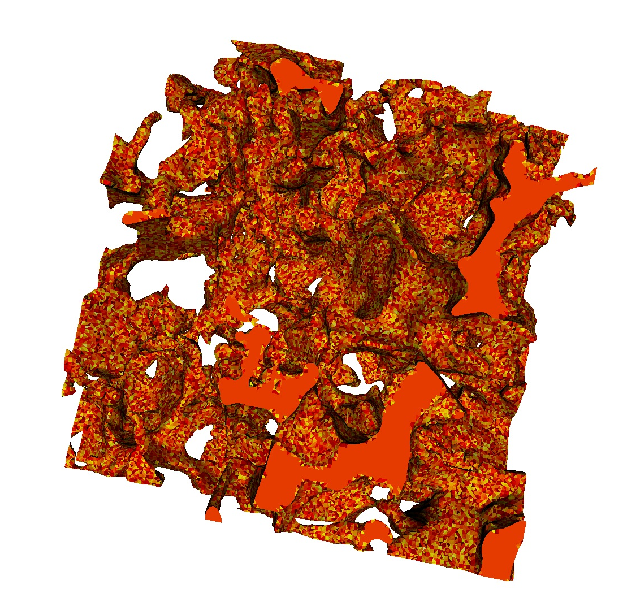
\includegraphics[width=\imagewidth]{berea-crop.pdf}
}

A close-up image reveals that it is composed of many\footnote{Millions, in fact} of small triangles forming tetrahedra:

{\centering
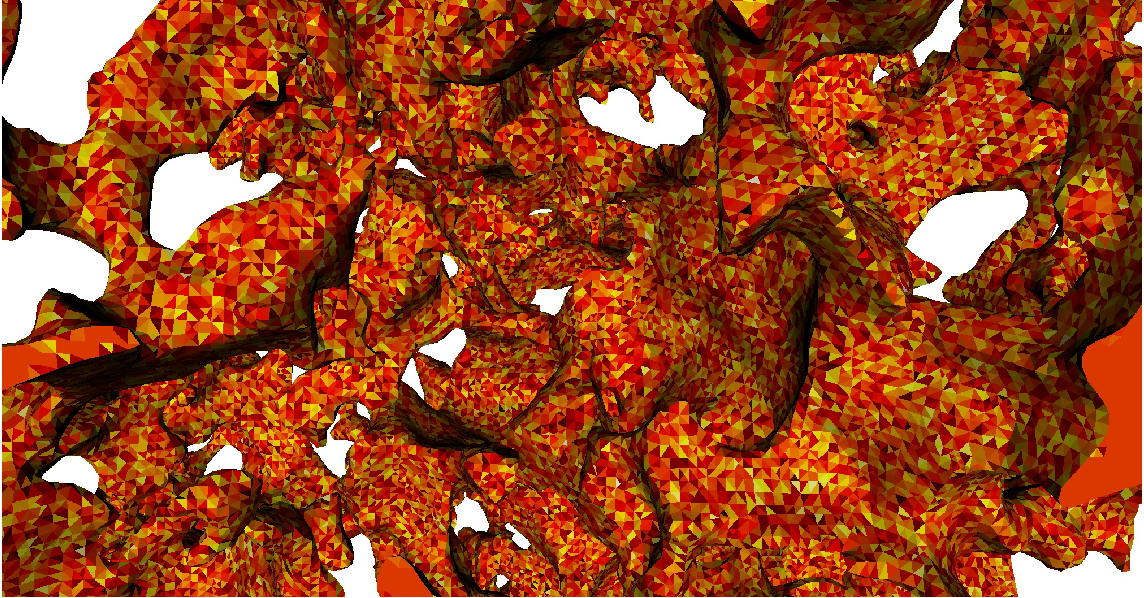
\includegraphics[width=\imagewidth]{berea-closeup-crop.pdf}
}


Suppose that we wish to compute the surface area of this mesh. For this two pieces of information are required:
\begin{itemize}
\item The position of each vertex in space.
\item The vertices that form each face; equivalently, the vertex connectivity.
\end{itemize}

This information may be represented generally with a data structure similar to the following:
%
%             |   |             |   |
%             |   |  /----n3--->|   | -> (x_1, y_1)
%             |   | /           |   |
% cell_id ->  |   |/------n1--->|   | -> (x_4, y_4)
%             |   |\            |   |
%             |   | \-----n4--->|   | -> (x_5, y_5)
%             |   |  \          |   |
%             |   |   \---n2--->|   | -> (x_12, y_12)
%             |   |             |   |
%             |   |             |   |
%             |   |             |   |
%           cell2nodes         node2coordinate

\begin{figure}[H]
\centering
\begin{tikzpicture}
% http://tex.stackexchange.com/questions/60897/arrows-between-two-tables
\matrix (A) [matrix of nodes,nodes={draw, minimum size=.65cm, text width=2cm,align=center}] at (0,1)
{
cell 0\\ cell 1\\ cell 2\\ cell 3\\ cell 4\\ cell 5\\
};

\matrix (B) [matrix of nodes,nodes={draw, minimum size=.65cm, text width=2cm,align=center}] at (7,1)
{
\emph{(-0.5,1)} \\ \emph{(1,-0.5)} \\ \emph{(-1,1)} \\ \emph{(-0.5,-1)} \\ \emph{(0.5,-0.5)} \\ \emph{(0.5,1)} \\ \emph{(0.5,0.5)} \\ \emph{(-1,-0.5)} \\ \emph{(-1,-1)} \\ \emph{(1,0.5)} \\ \emph{(-0.5,0.5)} \\ \emph{(-1,0.5)} \\ \emph{(-0.5,-0.5)} \\
};

\draw[->, -{Stealth[length=3mm]}] (A-1-1.east) -- (B-7-1.west);
\draw[->, -{Stealth[length=3mm]}] (A-1-1.east) -- (B-10-1.west);
\draw[->, -{Stealth[length=3mm]}] (A-1-1.east) -- (B-5-1.west);
\draw[->, -{Stealth[length=3mm]}] (A-1-1.east) -- (B-2-1.west);
\draw[->, -{Stealth[length=3mm]}] (A-2-1.east) -- (B-11-1.west);
\draw[->, -{Stealth[length=3mm]}] (A-2-1.east) -- (B-7-1.west);
\draw[->, -{Stealth[length=3mm]}] (A-2-1.east) -- (B-13-1.west);
\draw[->, -{Stealth[length=3mm]}] (A-2-1.east) -- (B-5-1.west);
\draw[->, -{Stealth[length=3mm]}] (A-3-1.east) -- (B-1-1.west);
\draw[->, -{Stealth[length=3mm]}] (A-3-1.east) -- (B-6-1.west);
\draw[->, -{Stealth[length=3mm]}] (A-3-1.east) -- (B-11-1.west);
\draw[->, -{Stealth[length=3mm]}] (A-3-1.east) -- (B-7-1.west);
\draw[->, -{Stealth[length=3mm]}] (A-4-1.east) -- (B-8-1.west);
\draw[->, -{Stealth[length=3mm]}] (A-4-1.east) -- (B-13-1.west);
\draw[->, -{Stealth[length=3mm]}] (A-4-1.east) -- (B-9-1.west);
\draw[->, -{Stealth[length=3mm]}] (A-4-1.east) -- (B-4-1.west);
\draw[->, -{Stealth[length=3mm]}] (A-5-1.east) -- (B-3-1.west);
\draw[->, -{Stealth[length=3mm]}] (A-5-1.east) -- (B-1-1.west);
\draw[->, -{Stealth[length=3mm]}] (A-5-1.east) -- (B-12-1.west);
\draw[->, -{Stealth[length=3mm]}] (A-5-1.east) -- (B-11-1.west);

\node (C) [below=.25cm of A]{Cells};
\node (C) [below=.25cm of B]{Vertex coordinates};
\end{tikzpicture}
\end{figure}


Notice how adjacent cells access vertices in a random fashion\footnote{Or at least random looking. The point is that there is clearly no structure.}. This is detrimental to performance for various reasons:

\begin{enumerate}
\item They exhibit weak spatial locality, a property which most modern CPU caches bank on to attain higher performance in IO bound applications, which may manifest through decisions regarding cache replacement strategies or data pre-fetching.
\item The indirection maps compete with valuable data for memory access as well as memory storage, both resulting in degraded cache performance.
\item Looking up addresses, as opposed to computing them directly, will typically prohibit or limit the scope of compiler-performed optimizations, not least vectorizations.
\end{enumerate}

Numerous strategies have been devoted to deal with this problem, notably applying a space filling curve to obtain a more favourable numbering, with closer elements tending to have closer numberings. While the space filling curve most certainly improves cache locality, it does not make use of more obvious structure that may exist. A mesh that is irregular and unstructured on the whole may contain subregions of high regularity and uniform structure, whose regularity/uniformity may be locally exploitable in a more direct manner, for potentially higher performance gains!


If on the other hand we look at a fully structured mesh such as this one:

\begin{figure}[H]
\centering
\includesvg[width=\imagewidth, svgpath=images/intro/]{fully-structured}
\end{figure}

As the vertices form a two-dimensional lattice, we can store their coordinates in a two-dimensional array such as the following:
\begin{figure}[H]
\centering
\begin{tabular}{|c|c|c|c|c|}
(2.0,8.9) & (3.9,8.4) & (5.9,7.9) & (7.9,7.4) & (9.9,6.9) \\
(1.4,6.8) & (3.3,6.4) & (5.3,6.0) & (7.3,5.5) & (5.3,4.9) \\
(0.7,4.9) & (2.7,4.5) & (4.7,4.1) & (6.7,3.6) & (4.6,3.1) \\
(0.0,2.9) & (2.1,2.6) & (4.2,2.4) & (6.2,2.0) & (8.2,2.5) \\
\end{tabular}
\end{figure}

The cells are now defined implicitly, one between each four vertices forming a quad! We need not explicitly store the mesh connectivity and computations can access the data directly without going through indirections.




\section{Contributions}

We present Crystal, a group of algorithms for \emph{extracting} regions of regularity in a mesh, reorganizing the mesh to \emph{expose} said structure in order to enable efficient \emph{exploitation}. The Crystal algorithms are embodied in a working prototype implementation.

We present a summary of our contributions, and discuss them in detail in what follows.

\begin{itemize}
\item Algorithms for extracting structure, and an evaluation of their competency.
\item Methodologies for reorganising the data layout to expose the structure, and a discussion about their relative merits.
\item A scheme for exploiting the structure efficiently, and a performance evaluation of its effectiveness.
\end{itemize}


\subsection{Extracting structure}
We formally define a notion of vertex structure in a mesh, in particular the properties that the vertex-vertex adjacency must exhibit within a structured region.


On this basis, a vertex structure extraction algorithm is devised and implemented. The algorithm traverses a constructed graph whose vertices correspond to the mesh's original vertices, and whose edges represent the vertex-vertex adjacency relation. Each structured region is ``grown'' from a given seed vertex, ensuring with each step that the extracted region is a well-formed structured region.

We also define the notion of a structured region for cells and edges, and develop algorithms for deriving said structure using previously extracted vertex structure.


\subsection{Exposing structure}
We describe how the underlying data storage layout must be reorganised to reflect the extracted structure and facilitate its exploitation. This must take into account elements within the unstructured regions, ensuring that accesses via the modified maps remain consistent with the originals.

\subsection{Exploiting structure}
Using the information gathered from the extracted structure, we can transform the data storage layout so as to implicitly represent the adjacency relationships between various mesh elements. This alleviates the need to use indirection maps when running computations over a structured region, substituting them for a small constant amount of meta-data per structured region that is used to define each region's dimensions and orientation. Computations over an unstructured region execute as normal using restructured versions of the original maps and data.

This allows us to transform a cell-to-nodes access operation from the following, which uses indirections to access the node data:
\begin{lstlisting}[language=c++]
for (int cell_id = 0 ; cell_id < num_cells ; ++cell_id) {
	int node0 = cell_to_nodes[cell_id][0];
	int node1 = cell_to_nodes[cell_id][1];
	int node2 = cell_to_nodes[cell_id][2];
	int node3 = cell_to_nodes[cell_id][3];

	int node0_data = data[node0];
	int node1_data = data[node1];
	int node2_data = data[node2];
	int node3_data = data[node3];

	// Use data
}
\end{lstlisting}

To something like this, which computes the location of node data directly:
% SEE https://gmplib.org/~tege/x86-timing.pdf
\begin{lstlisting}[language=c++]
for (int row = 0 ; row < num_rows ; ++row) {
	for (int col = 0 ; col < num_cols ; ++col) {
		int node0 = row * nodes_per_row + col;
		int node1 = row * nodes_per_row + (col+1);
		int node2 = (row+1) * nodes_per_row + col;
		int node3 = (row+1) * nodes_per_row + (col+1);

		int node0_data = data[node0];
		int node1_data = data[node1];
		int node2_data = data[node2];
		int node3_data = data[node3];

		// Use data
	}
}
\end{lstlisting}


\subsection{Unfinished Sentences...}
In particular, we present and evaluate an implementation for extracting and exposing structure in quadrilateral meshes on various examples, and evaluate a 33\% performance improvement achieved by exploiting the structure on the airfoil computation.
